\chapter{Vergleich der Verifizierung von Implementierungen}

Nachdem im vorigen Kapitel die Spezifikationen und darin verwendete Sprachmittel verglichen wurden,
geht es nun darum zu verifizieren, dass die Implementierungen diese tatsächlich erfüllen.
Die Werkzeuge Verifast bzw. ACSL führen dazu eigene Berechnungen durch, benötigen aber dennoch
zusätzliche Annotationen im Quellcode, damit die korrekten logische Schlüsse gezogen 
werden können. Beispielsweise müssen Schleifeninvarianten ergänzt werden oder sogenannte
Ghost-Commands, die Prädikate oder weitere logische Beweise mit einbeziehen.

\section{Symbolische Ausführung in Verifast}

Die Verifizierung von Implementierungs-Code findet in Verifast über eine symbolische Ausführung statt:
Gestartet wird mit den Vorbedingungen des Methodenvertrags, der Code wird dann wie bei der tatsächlichen
Ausführung von oben nach unten verarbeitet. Jedoch nicht mit konkreten, sondern mit 
abrakten Werten. Diese werden durch logische Formeln repräsentiert, welche die möglichen Variablen-Werte 
beschreiben. Am Ende der Ausführung sind dann bei erfolgreicher Verifizierung alle Voraussetzungen
erfüllt, um die Nachbedingungen direkt abzuleiten.
\newline
\newline
Bei der symbolischen Ausführung werden alle potenziellen Ausführungspfade untersucht: Schleifen
oder auch \texttt{if}-Anweisungen sorgen dafür, dass Verifast diese Verzweigungen einzeln betrachtet
und verifiziert. Existieren z.B. mehrere \texttt{return}-Anweisungen in der Implementierung, so stellt
das Werkzeug sicher, dass in jedem Ausgang die Nachbedingungen gelten.

\begin{SCfigure}[1.7][h!]
	\centering
		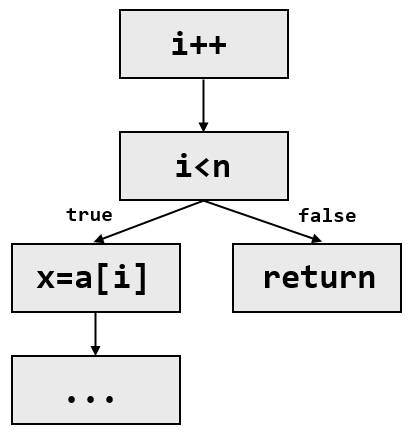
\includegraphics[width=0.3\textwidth]{images/symbolic_execution.png}
		\caption{Ausführungspfade für die symbolische Ausführung einer if-Anweisung}
\end{SCfigure}

Der aktuelle Zustand der Ausführung wird dabei durch zwei verschiedene Strukturen charakterisiert: 
Den Heap, der alle Elemente (engl. heap chunks) des Speichers beinhaltet sowie eine Liste
der geschlussfolgerten Annahmen (engl. assumptions). Bei der Ausführung der Vorbedingungen werden
diese Aussagen nun untersucht und entweder zum Heap hinzugefügt oder zu den Annahmen.

Beim Verstehen dieser Schritte ist die Verifast-Oberfläche sehr hilfreich, da sie den aktuellen
Zustand für einen beliebigen Haltepunkt anzeigen kann. Die folgende Situation zeigt die Ausführung
einer \lstinline{mismatch}-Implementierung bis zum gesetzten Haltepunkt (gelb hervorgehoben).

\begin{center}
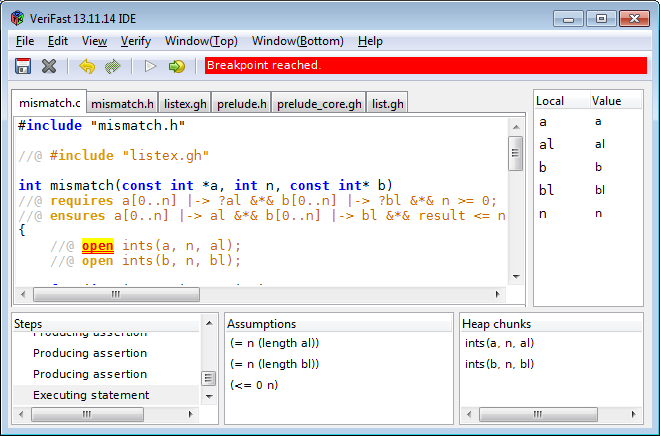
\includegraphics[width=1.0\textwidth]{images/verifast-state-after-precondition.png}
\end{center}

Gut zu erkennen ist, dass logische Ausdrücke wie \(n >= 0\) in die Liste der Annahmen 
(im Bild als \glqq Assumptions\grqq betitelt) aufgenommen wurden. Die \lstinline{ints}-Prädikate hingegen
wurden zum Heap hinzugefügt. Diesen Prozess nennt Verifast \glqq Producing assertion\grqq, wobei sich das Verb
\glqq Producing\grqq auf das Hinzufügen von Elementen zum aktuellen Zustand der symbolischen Ausführung
bezieht.

Das Gegenteil - \glqq Consuming assertion\grqq - findet z.B. beim Verifizieren der Nachbedingungen statt.
Verifast versucht dann alle erforderlichen Aussagen in der Liste der Annahmen bzw. im Heap zu finden
und diese, wenn sie denn passen, zu entfernen. Zusätzlich dazu wird am Ende einer Funktion - beim 
\glqq Leak check\grqq - auch überprüft, dass der Heap (der aktuellen Funktion) leer ist. Ist das nicht 
der Fall so wurde der entsprechende Speicher nicht korrekt bereinigt oder zumindest war Verifast nicht 
in der Lage das Gegenteil zu beweisen.

In dem Fall von mismatch würde Verifast die Heap chunks \lstinline{ints(a, n, al)} sowie
\lstinline{ints(b, n, bl)} beim Konsumieren der Nachbedingung auf dem Heap finden, entfernen und
somit erfolgreich verifizieren können, dass der Speicher so wie vor dem Aufruf vorhanden ist.



\section{Assertions und Ghost-Commands}

Zusicherungen (engl. assertions) und Ghost-Commands sind Annotationen, die direkt in den Implementierungs-Code
geschrieben werden. Assertions stellen sicher, dass der enthaltene Ausdruck wahr ist und sind ein nützliches Hilfsmittel, 
um die Verifizierung besser nachzuvollziehen als auch verständlicher zu machen. Insbesondere dann, wenn das Verifikationswerkzeug 
nicht triviale Schlüsse zieht, ist es von Vorteil Assertions zu ergänzen und im Code zu belassen.

Ghost-Commands hingegen enthalten Anweisungen für die Verifizierung, z.B. das Aufrufen anderer Sprachkonstrukte 
(z.B. Lemmata oder Fixpointfunktionen, siehe \ref{verifizierung:lemma}). Sie helfen dem Werkzeug logische Schlüsse 
zu ziehen, die es alleine nicht tun kann.
\newline
\newline
Der folgende Quellcode zeigt einen Ausschnitt aus einer rekursiven Implementierung für \lstinline{equal} und dient
hier als Anschauungsmaterial für die Erklärung der oben genannten Annotationstypen:

\lstinputlisting[language=C, caption=Rekursive Implementierung für \lstinline{equal} mit Verifast]{codes/equal_recursive_verifast.c}

Diese Implementierung zeigt nur die Abbruchbedingung der Rekursion - ist \lstinline{n == 0}, so sind die
leeren Listen gleich und die Berechnung terminiert. 

Die Zeilen 9 und 10 sind Assertions, die formal beschreiben, dass die induktiven Listen \lstinline{al} und
\lstinline{bl} die Länge 0 haben müssen und somit gleich lang sind. Damit Verifast in der Lage ist das zu
beweisen sind die zwei Ghost-Commands in Zeile 5 und 6 notwendig. Sie öffnen das \lstinline{ints}-Prädikat
und bringen somit dessen Inhalt in die Liste der Annahmen. Erst dadurch ist für Verifast ersichtlich, dass 
\lstinline{n} gleichzusetzen ist mit \texttt{length(al)} und \texttt{length(bl)}. Außerdem produziert
das Öffnen des Prädikats die Formel \lstinline{al = nil} bzw. \lstinline{bl = nil} (siehe Definition
des Prädikats in Listing 3.9 oder 4.2). Damit löst sich die Assertion \lstinline{al == bl} in den
trivialen Vergleich \lstinline{nil == nil} auf.
\newline
\newline
Das Öffnen der Prädikate konsumiert gleichzeitig auch die entsprechenden Heap-Chunks, was jedoch dazu führt,
dass diese beim Produzieren der Nachbedingung fehlen. Sie müssen also vor der \(return\)-Anweisung
wieder geschlossen werden (Zeile 11 und 12), damit sie dann wieder an den Aufrufer zurückgegeben werden können 
- so wie es die Nachbedingung verlangt.

Das Schreiben dieser \(close\)-Annotation ist jedoch oft nicht notwendig, da Verifast sie automatisch
einführt, wenn es sich um ein sogenanntes präzises Prädikat handelt. Darunter versteht Verifast Prädikate mit 
eingehenden und ausgehenden Parametern, die exakt die gleiche Speicherregion repräsentieren. 

\begin{figure}[H]
Die Kennzeichnung als präzises Prädikat geschieht über die Nutzung eines Semikolons bei der Trennung
der Prädikaten-Parameter:

\lstinputlisting[language=C, caption=Präzises Prädikat \lstinline{ints}]{codes/ints_precise_predicate_verifast.c}
\end{figure}
Präzise Prädikate versucht Verifast während der Verifizierung automatisch zu öffnen und ggf. auch zu
schließen. Dadurch ist in der obigen Implementierung das Schreiben der \texttt{close}-Anweisungen
nicht zwingend notwendig.
\newline
\newline
Assertions in ACSL werden genauso notiert wie in Verifast. Ghost-Commands hingegen werden
mit dem Schlüsseltwort \lstinline{ghost} eingeleitet, sind aber generell nicht so oft wie in
Verifast notwendig. Das kommt daher, dass Frama-C aufwendigere Berechnungen durchführt, um
entsprechende logische Schlüsse zu ziehen. Das ist jedoch auch spürbar, wenn man die
Geschwindigkeit der Werkzeuge vergleicht.


\section{Schleifeninvarianten}

Schleifeninvarianten beschreiben eine Eigenschaft, die vor und nach jeder Iteration gültig ist. Sie
werden wie Ghost-Commands per Annotation an die Schleife geschrieben und helfen dem Werkzeug die
Nachbedingungen zu verifizieren.

\begin{figure}[H]
Der folgende Quellcode zeigt eine ACSL-Implementierung für \lstinline{mismatch}
(Spezifikation siehe Listing 3.11):
\lstinputlisting[language=C, caption=Implementierung für \lstinline{mismatch} mit ACSL-Annotationen]{codes/mismatch_acsl.c}
\end{figure}

Die Invariante in Zeile 4 beschreibt den Gültigkeitsbereich der Variable \lstinline{i}, in Zeile 5 wird definiert, 
dass alle Elemente \lstinline{< i } der beiden Arrays gleich sind. Außerdem verlangt ACSL, dass alle
Variablen-Manipulationen für die Schleife explizit angegeben werden (siehe Zeile 6). Damit kann das Werkzeug
nun die beiden Fälle aus den Nachbedingungen beweisen.

Hier erweist es sich auch wieder als vorteilhaft, dass für die Spezifikation bereits das Prädikat
\lstinline{IsEqual} definiert wurde, denn in der Schleifeninvariante kann dieses wiederverwendet werden. Damit
ist auch für den Leser schneller ersichtlich, dass die Invariante beim Beweis der Spezifikation hilft.

\begin{figure}[H]
	\centering
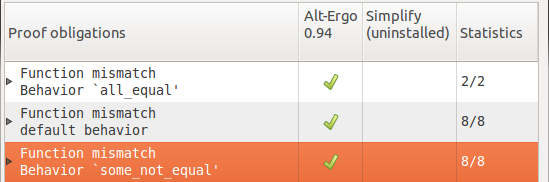
\includegraphics[width=0.8\textwidth]{images/acsl-prove-mismatch.png}

Die Implementierung für \lstinline{mismatch} wurde erfolgreich verifiziert.
\end{figure}

Invarianten in ACSL und Verifast funktionieren bis auf kleinere syntaktische Unterschiede nach dem gleichen Prinzip.
Wie schon von den Spezifikationen bekannt, ist es auch hier in Verifast wieder notwendig die Invarianten in nur
einer einzigen Annotation auszudrücken. Außerdem kann der Schleifenkörper nur auf Heap-Chunks zurückgreifen, die
in der Invariante explizit angegeben werden. Verifast entfernt vor dem Schleifenbeginn alle aktuellen Chunks
und stellt diese nach dem Austritt aus der Schleife wieder her. Der Schleifenkörper verhält sich also
wie eine eigenständige Funktion.

\begin{figure}[H]
Nachfolgend ist die Implementation von oben nochmal gezeigt, an der Stelle aber mit Invarianten für Verifast.

\lstinputlisting[language=C, caption=Implementierung für \lstinline{mismatch} mit Verifast-Annotationen]{codes/mismatch_verifast.c}
\end{figure} 

Wie in der dazugehörigen Spezifikation (siehe Listing 3.10) wird die Funktion \lstinline{take} genutzt,
um die ersten \lstinline{i} Elemente der Liste \lstinline{al} und \lstinline{bl} zu vergleichen.
Die Einschränkung des Wertebereichs der Variablen \lstinline{i} ist identisch mit der ACSL-Variante -
bis auf den syntaktischen Unterschied, dass Verifast keine Verkettung von Vergleichsoperatoren erlaubt.

Wie oben beschrieben muss außerdem der Speicherinhalt der Arrays \lstinline{al} und \lstinline{bl} für
den Schleifenkörper zugreifbar gemacht werden. Deshalb finden sich hier die \lstinline{ints}-Prädikate
aus der Spezifikation wieder. Sie stellen sicher, dass die Elemente \lstinline{a[0 <= i < n]} gelesen
werden können.

Im Unterschied zu Verifast ist es nicht notwendig und auch nicht möglich Schreibrechte für die lokale Variable 
\lstinline{i} zu erteilen. Auf lokale Variablen darf der Schleifenkörper in Verifast immer zugreifen, lesend
als auch schreibend.
\newline
\newline
Versucht man die Implementierung mit Verifast nun zu beweisen, erhält man einen Fehler: Die Schleifeninvariante
konnte nicht bewiesen werden. 
Das liegt daran, dass das Werkzeug aus dem Schleifenkörper allein nicht folgern kann, dass in der nächsten Iteration 
die Länge der gleichen Listen um eins gewachsen ist. Der Fehler tritt darum beim \lstinline{==} der Invariante auf.
Zur Lösung wird ein Lemma benötigt, welchen diesen Schritt für Verifast nachvollziehbar macht.

\section{Lemmata und Axiome}
\label{verifizierung:lemma}

detailliert zeigen wie der schritt gemacht werden kann

take(i, al) und take(i, bl) und a[i] == b[i] daraus folgt take(i + 1, al) == take(i + 1, bl)

take_one_plus lemma zeigen

man muss die lemmas alle kennen .. oder selber schreiben

es zeigt sich wieder: verifast wertet geschwindigkeit wichtiger als intelligenz des werkzeugs

automatische ausführen von lemmas geht mit lemma_auto

wurde tatsächlich schon automatisch benutzt ... kann auch gut mit der verifast gui nachfollzogen werden
beim ints prädikat

intsinv zeigen mit length

lemma auto ist axiom

erwähnen dass verifast terminierung von fixpount und lemmas prüft


\section{Speicherprobleme aufdecken}

malloc/free - chunks

zeigen an hand von main-funktion (unit-test)

verifast hilft klar zu dokumentieren wer für speicher verantwortlich ist (rufer oder gerufener)

\section{Überläufe erkennen}

overflow checken
